% quick_ref.tex

%%%%%%%%%%%%%%%%%%%%%%%%%%%%%%%%%%%%%%%%%%%%%%%%%%%%%%%%%%%%
\SUBSECTION{Quick reference guide}
%%%%%%%%%%%%%%%%%%%%%%%%%%%%%%%%%%%%%%%%%%%%%%%%%%%%%%%%%%%%

\subsubsection*{Examples}

To get familiar with \CosmoPMC, use the examples which are contained
in the package. Simply change to one of the subdirectories in
\direc{\COSMOPMCDIR/Demo/MC\_Demo} and proceed on to the point
\textbf{Run} below.

\subsubsection*{User-defined runs}

To run different likelihood combinations, or your own data, the
following two steps are necessary to set up a \CosmoPMC\ run.

\begin{enumerate}

   \item \textbf{Data and parameter files}

     Create new directory with
     \ttrefc{newdirpmcsh}{newdir\_pmc.sh}{\thenewdirpmcshc}.  When
     asked, enter the likelihood/data type. More than one type can be
     chosen by adding the corresponding (bit-coded) type
     id's. Symbolic links to corresponding files in
     \direc{\COSMOPMCDIR/data} are set, and parameter files from
     \direc{\COSMOPMCDIR/par\_files} are copied to the new directory
     on request.

     If necessary, copy different or additional data and/or parameter
     files to the present directory.


    \item \textbf{Configuration file}

      Create the PMC configuration file \file{config\_pmc}. Examples
      for existing data modules can be
      found in \direc{\COSMOPMCDIR/Demo/MC\_Demo}\REF{, see also
      Sect.~}{sec:config_file}{ for details}.

      In some cases, information about the galaxy redshift
      distribution(s) have to be provided, and the corresponding files
      copied (see \direc{\COSMOPMCDIR/Demo} for example files
      `\file{nofz*}').

    \end{enumerate}


\subsubsection*{Run}

Type
%
\command{\$COSMOPMC/bin/cosmo\_pmc.pl -n NCPU}
%
to run \CosmoPMC\ on \texttt{NCPU} CPUs. See
`\ttrefc{cosmopmcpl}{cosmo\_pmc.pl}{\thecosmopmcplc} \progr{-h}' for
more options. Depending on the type of initial proposal\REF{ (Sect.~}{sec:ini_prop}{)},
a maximum-search is started followed by a
Fisher matrix calculation. After that, PMC is
started. Fig.~\ref{fig:cosmo_pmc_flow} shows a flow chart of the
script's actions.


\subsubsection*{Diagnostics}

Check the files \file{perplexity} and
\file{enc}. If the perplexity reaches values of 0.8 or larger, and
if the effective number of components (ENC) is not smaller than 1.5,
the posterior has very likely been explored sufficiently. Those and
other files are updated during run-time and can be monitored while PMC
is running. \REF{See Sect.~}{sec:diagnostics}{\ for more details.}


\subsubsection*{Results}

The text file \file{iter\_\{niter-1\}/mean} contains mean and
confidence levels. The file \\
\file{iter\_\{niter-1\}/all\_contour2d.pdf} shows the 1d- and
2d-marginals. Plots can be redone or refined, or created from other
than the last iteration with
\ttrefc{plotcontourzdpl}{plot\_contour2d.pl}{\theplotcontourzdplc}.
Note that in the default setting, the posterior plots are not
smoothed. \REF{See Sect.~}{sec:marginal_plots}{\ for more details}, and
for information on the alternative script
\ttrefc{plotconfidenceR}{plot\_confidence.R}{\theplotconfidenceRc}.

\begin{figure}[!tb]
  
  \begin{center}
   \resizebox{\hsize}{!}{
     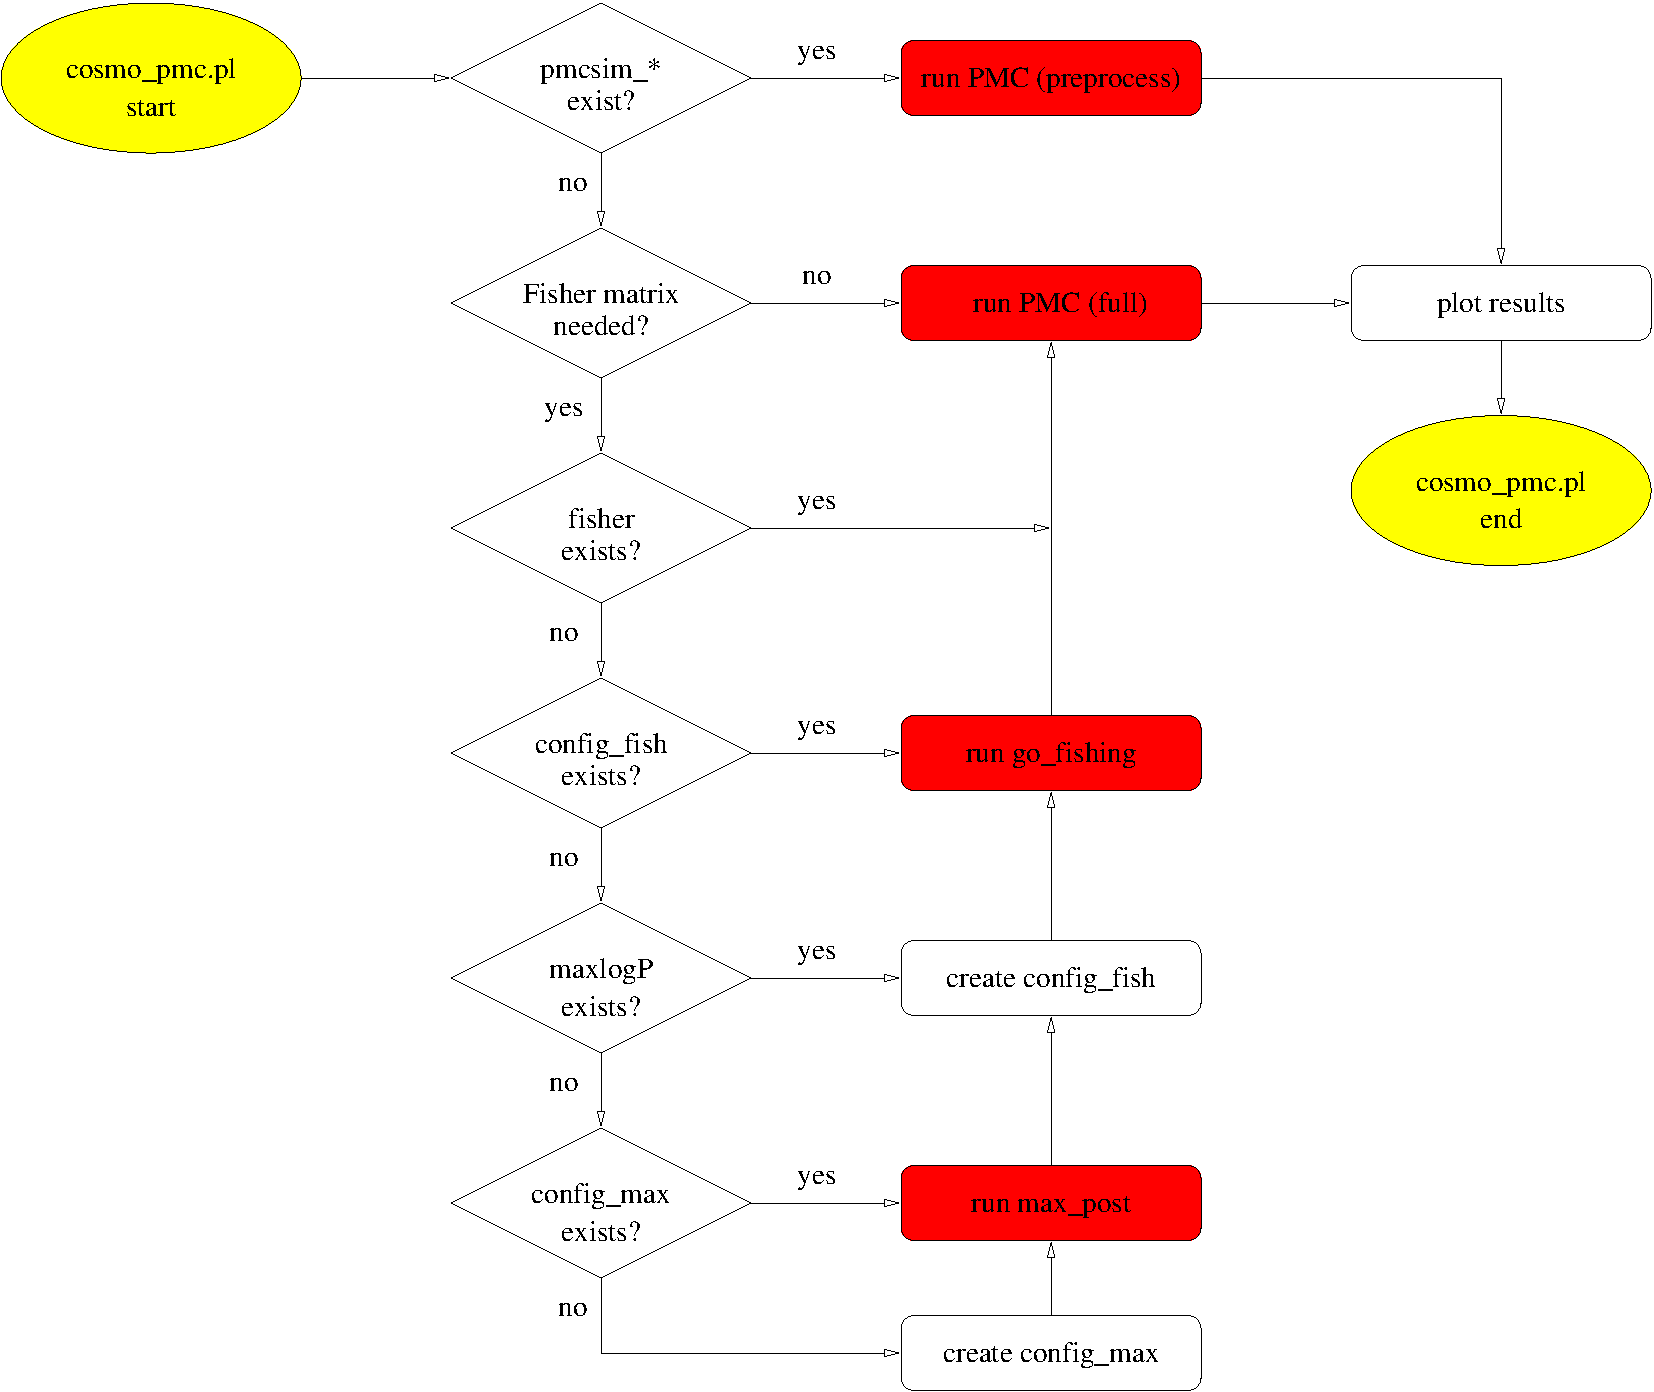
\includegraphics{cosmo_pmc_flow}
    }
  \end{center}
  
  \caption{Flow chart for \progr{cosmo\_pmc.pl}.} %\ttrefc{cosmopmcpl}{cosmo\_pmc.pl}{\thecosmopmcplc}.}
  \label{fig:cosmo_pmc_flow}
\end{figure}

